\documentclass[12pt,landscape]{article}
\usepackage[margin=0.5in]{geometry}
\usepackage{tikz}
\usetikzlibrary{shapes,arrows,positioning,calc,fit,backgrounds}
\usepackage{amsmath}
\usepackage{xcolor}

\definecolor{inputcolor}{RGB}{52,152,219}
\definecolor{hiddencolor}{RGB}{46,204,113}
\definecolor{outputcolor}{RGB}{231,76,60}
\definecolor{physicscolor}{RGB}{155,89,182}
\definecolor{datacolor}{RGB}{241,196,15}

\begin{document}

% Diagram 1: Complete PINN Architecture
\begin{figure}[p]
\centering
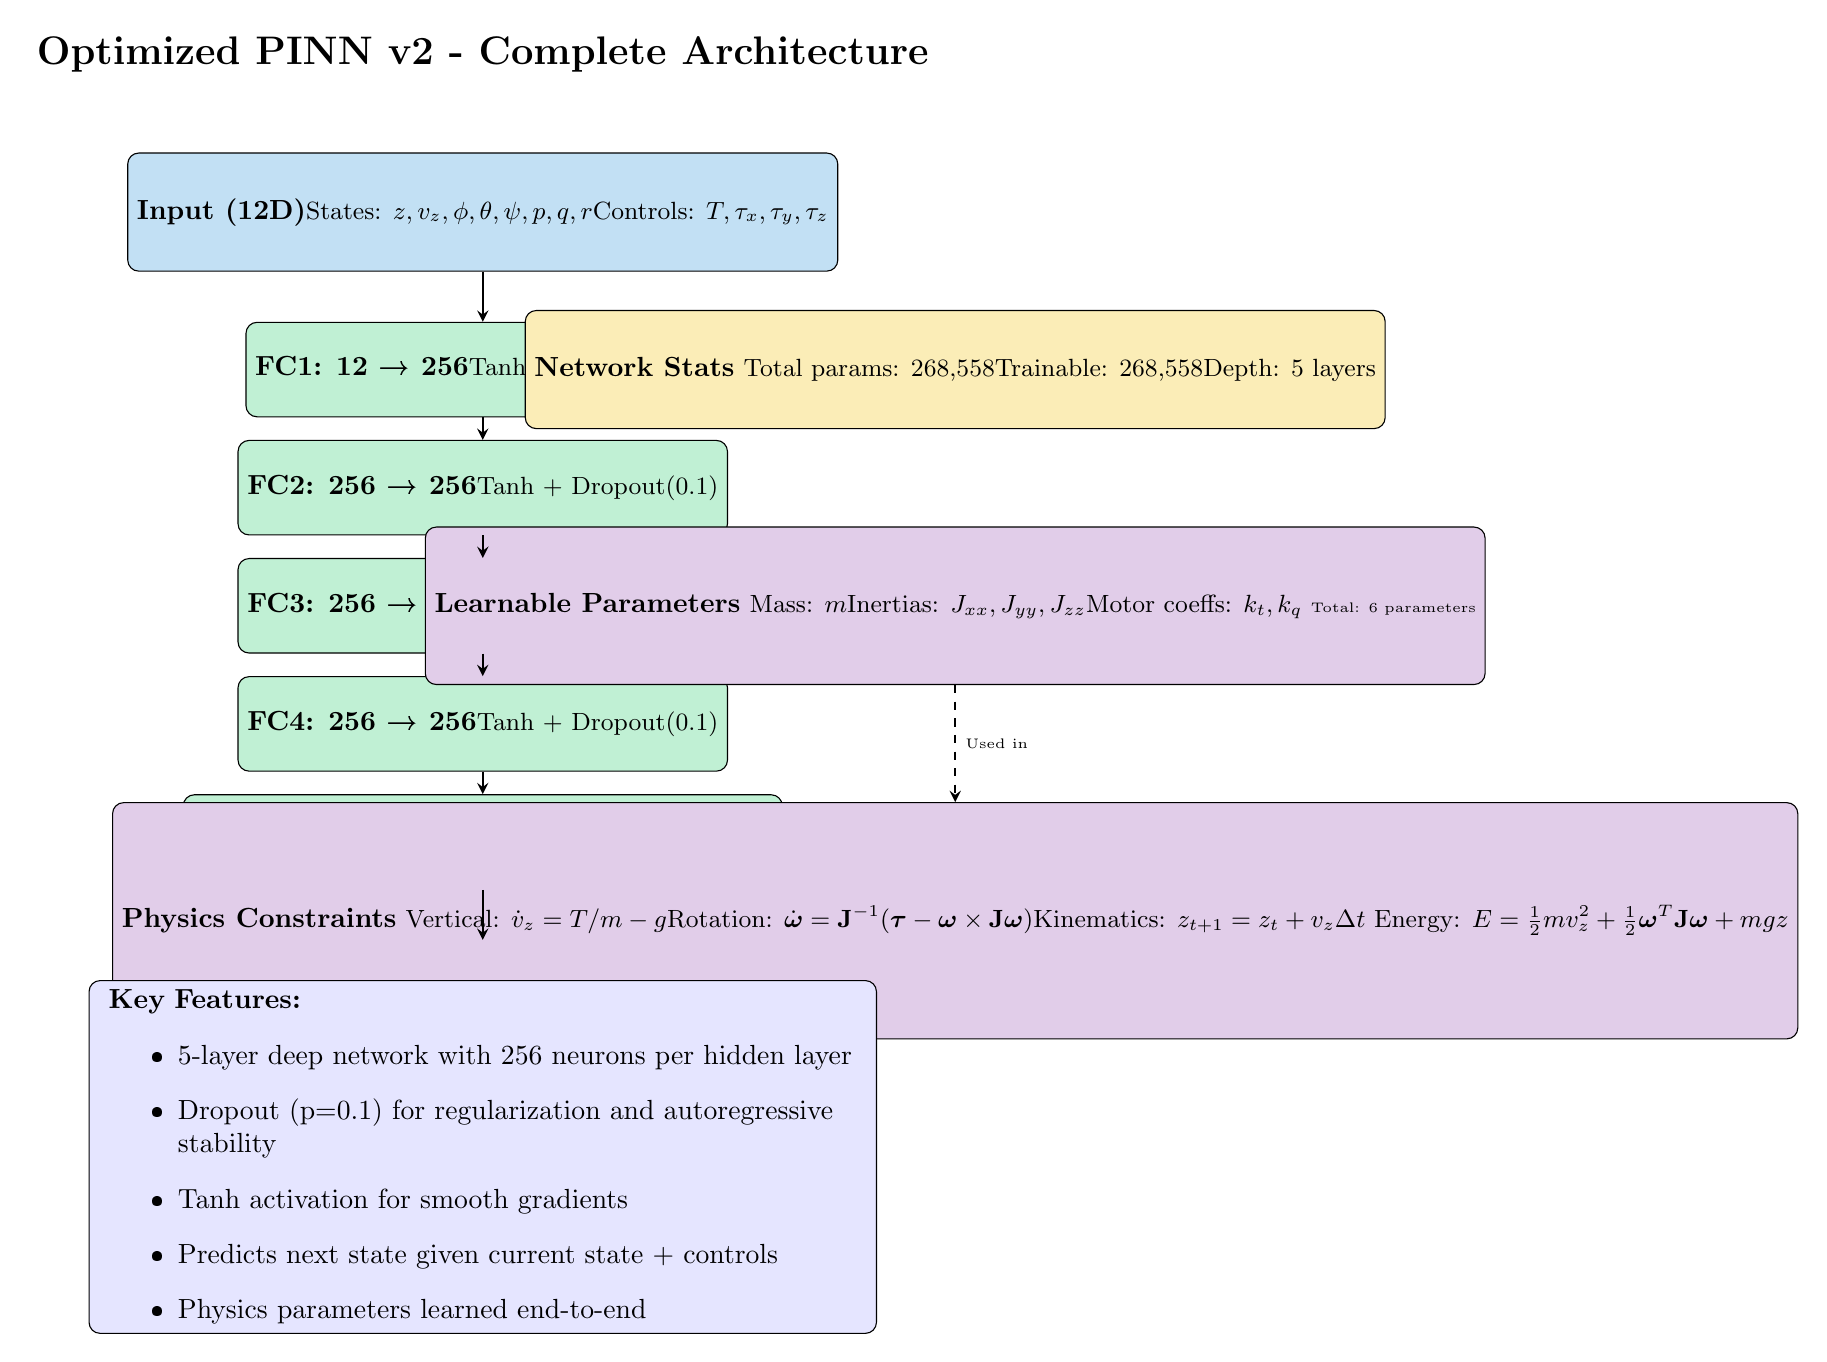
\begin{tikzpicture}[
    box/.style={rectangle, draw, minimum width=2cm, minimum height=1cm, text centered, rounded corners},
    layer/.style={box, fill=hiddencolor!30},
    input/.style={box, fill=inputcolor!30},
    output/.style={box, fill=outputcolor!30},
    physics/.style={box, fill=physicscolor!30},
    data/.style={box, fill=datacolor!30},
    arrow/.style={->, >=stealth, thick}
]

% Title
\node[font=\Large\bfseries] at (0,10) {Optimized PINN v2 - Complete Architecture};

% Input layer
\node[input, minimum width=3cm, minimum height=1.5cm] (input) at (0,8) {
    \textbf{Input (12D)}\\
    \small
    States: $z, v_z, \phi, \theta, \psi, p, q, r$\\
    Controls: $T, \tau_x, \tau_y, \tau_z$
};

% Hidden layers
\node[layer, minimum width=4cm, minimum height=1.2cm] (fc1) at (0,6) {
    \textbf{FC1: 12 → 256}\\
    \small Tanh + Dropout(0.1)
};

\node[layer, minimum width=4cm, minimum height=1.2cm] (fc2) at (0,4.5) {
    \textbf{FC2: 256 → 256}\\
    \small Tanh + Dropout(0.1)
};

\node[layer, minimum width=4cm, minimum height=1.2cm] (fc3) at (0,3) {
    \textbf{FC3: 256 → 256}\\
    \small Tanh + Dropout(0.1)
};

\node[layer, minimum width=4cm, minimum height=1.2cm] (fc4) at (0,1.5) {
    \textbf{FC4: 256 → 256}\\
    \small Tanh + Dropout(0.1)
};

\node[layer, minimum width=4cm, minimum height=1.2cm] (fc5) at (0,0) {
    \textbf{FC5 (Output): 256 → 8}\\
    \small Linear (no activation)
};

% Output
\node[output, minimum width=3cm, minimum height=1.5cm] (output) at (0,-2) {
    \textbf{Predicted States}\\
    \small $\hat{z}, \hat{v}_z, \hat{\phi}, \hat{\theta}, \hat{\psi}, \hat{p}, \hat{q}, \hat{r}$
};

% Learnable parameters (side)
\node[physics, minimum width=3.5cm, minimum height=2cm] (params) at (6,3) {
    \textbf{Learnable Parameters}\\[0.2cm]
    \small
    Mass: $m$\\
    Inertias: $J_{xx}, J_{yy}, J_{zz}$\\
    Motor coeffs: $k_t, k_q$\\[0.1cm]
    \tiny Total: 6 parameters
};

% Physics computation
\node[physics, minimum width=5cm, minimum height=3cm] (physics_comp) at (6,-1) {
    \textbf{Physics Constraints}\\[0.2cm]
    \small
    Vertical: $\dot{v}_z = T/m - g$\\
    Rotation: $\dot{\boldsymbol{\omega}} = \mathbf{J}^{-1}(\boldsymbol{\tau} - \boldsymbol{\omega} \times \mathbf{J}\boldsymbol{\omega})$\\
    Kinematics: $z_{t+1} = z_t + v_z \Delta t$\\[0.1cm]
    Energy: $E = \frac{1}{2}mv_z^2 + \frac{1}{2}\boldsymbol{\omega}^T\mathbf{J}\boldsymbol{\omega} + mgz$
};

% Arrows
\draw[arrow] (input) -- (fc1);
\draw[arrow] (fc1) -- (fc2);
\draw[arrow] (fc2) -- (fc3);
\draw[arrow] (fc3) -- (fc4);
\draw[arrow] (fc4) -- (fc5);
\draw[arrow] (fc5) -- (output);

\draw[arrow, dashed] (params) -- (physics_comp) node[midway, right, font=\tiny] {Used in};
\draw[arrow, dashed, red] (output) -- (physics_comp) node[midway, below, font=\tiny] {Verified by};

% Parameter count box
\node[data, minimum width=3.5cm, minimum height=1.5cm] (param_count) at (6,6) {
    \textbf{Network Stats}\\[0.2cm]
    \small
    Total params: 268,558\\
    Trainable: 268,558\\
    Depth: 5 layers
};

% Info boxes
\node[draw, rounded corners, fill=blue!10, minimum width=10cm, text width=9.5cm] at (0,-4) {
    \textbf{Key Features:}
    \begin{itemize}
        \item 5-layer deep network with 256 neurons per hidden layer
        \item Dropout (p=0.1) for regularization and autoregressive stability
        \item Tanh activation for smooth gradients
        \item Predicts next state given current state + controls
        \item Physics parameters learned end-to-end
    \end{itemize}
};

\end{tikzpicture}
\end{figure}

\clearpage

% Diagram 2: Training Pipeline with Curriculum Learning
\begin{figure}[p]
\centering
\begin{tikzpicture}[
    box/.style={rectangle, draw, minimum width=2.5cm, minimum height=1cm, text centered, rounded corners},
    phase/.style={box, fill=blue!20},
    process/.style={box, fill=green!20},
    loss/.style={box, fill=red!20},
    arrow/.style={->, >=stealth, thick}
]

\node[font=\Large\bfseries] at (6,10) {Training Pipeline: Curriculum Learning \& Multi-Step Rollout};

% Phase timeline
\node[phase, minimum width=4cm, minimum height=1.5cm] (phase1) at (0,8) {
    \textbf{Phase 1: Epochs 0-50}\\
    \small 5-step rollouts\\
    Easy: Short horizon
};

\node[phase, minimum width=4cm, minimum height=1.5cm] (phase2) at (4,8) {
    \textbf{Phase 2: Epochs 50-100}\\
    \small 10-step rollouts\\
    Medium difficulty
};

\node[phase, minimum width=4cm, minimum height=1.5cm] (phase3) at (8,8) {
    \textbf{Phase 3: Epochs 100-150}\\
    \small 25-step rollouts\\
    Harder
};

\node[phase, minimum width=4cm, minimum height=1.5cm] (phase4) at (12,8) {
    \textbf{Phase 4: Epochs 150-230}\\
    \small 50-step rollouts\\
    Full difficulty
};

\draw[arrow] (phase1) -- (phase2);
\draw[arrow] (phase2) -- (phase3);
\draw[arrow] (phase3) -- (phase4);

% Scheduled sampling
\node[process, minimum width=12cm, minimum height=1.2cm] (sched_samp) at (6,6) {
    \textbf{Scheduled Sampling}: Linearly increase 0\% → 30\%\\
    \small Use predicted states instead of ground truth with probability $p$
};

\draw[arrow, dashed] (phase1.south) -- (sched_samp.north);
\draw[arrow, dashed] (phase2.south) -- (sched_samp.north);
\draw[arrow, dashed] (phase3.south) -- (sched_samp.north);
\draw[arrow, dashed] (phase4.south) -- (sched_samp.north);

% Multi-step rollout visualization
\node[font=\large\bfseries] at (6,4.5) {Multi-Step Autoregressive Rollout};

\foreach \i in {0,1,2,3,4} {
    \node[box, fill=inputcolor!30, minimum width=1.5cm, minimum height=0.8cm] (state\i) at (1.5*\i,3.2) {$x_{\i}$};
    \node[box, fill=hiddencolor!30, minimum width=1.5cm, minimum height=0.5cm] (model\i) at (1.5*\i,2) {NN};

    \ifnum\i<4
        \node[box, fill=outputcolor!30, minimum width=1.5cm, minimum height=0.8cm] (pred\i) at (1.5*\i+1.5,3.2) {$\hat{x}_{\the\numexpr\i+1}$};
        \draw[arrow] (state\i) -- (model\i);
        \draw[arrow] (model\i) -- (pred\i);
        \draw[arrow, dashed, blue] (pred\i) -- (state\the\numexpr\i+1);
    \fi
}

\node[font=\small] at (6,1.2) {
    Each prediction feeds into next timestep (autoregressive)
};

% Loss components
\node[loss, minimum width=3cm, minimum height=1cm] (loss_data) at (1,0) {
    \textbf{Data Loss}\\
    \small $||\hat{x} - x||^2$
};

\node[loss, minimum width=3cm, minimum height=1cm] (loss_physics) at (4.5,0) {
    \textbf{Physics Loss}\\
    \small $||f(\hat{x}) - 0||^2$
};

\node[loss, minimum width=3cm, minimum height=1cm] (loss_rollout) at (8,0) {
    \textbf{Rollout Loss}\\
    \small $\sum_{k=1}^{K} \frac{1}{k}||\hat{x}_k - x_k||^2$
};

\node[loss, minimum width=3cm, minimum height=1cm] (loss_energy) at (11.5,0) {
    \textbf{Energy Loss}\\
    \small $(E_{pred} - E_{true})^2$
};

% Final optimizer phase
\node[phase, minimum width=12cm, minimum height=1.2cm] (lbfgs) at (6,-1.5) {
    \textbf{Phase 5: L-BFGS Fine-tuning (Epochs 230-250)}\\
    \small Full-batch second-order optimization for final convergence
};

\draw[arrow] (phase4.south) -- ++(0,-3.5);

\end{tikzpicture}
\end{figure}

\clearpage

% Diagram 3: Physics Integration - How Physics Constraints Work
\begin{figure}[p]
\centering
\begin{tikzpicture}[
    box/.style={rectangle, draw, minimum width=2.5cm, minimum height=1cm, text centered, rounded corners},
    eqbox/.style={box, fill=yellow!20, minimum width=8cm, minimum height=1.2cm},
    arrow/.style={->, >=stealth, thick}
]

\node[font=\Large\bfseries] at (6,10) {Physics-Informed Neural Network: Loss Computation};

% Current state
\node[input, minimum width=3cm, minimum height=1.5cm] (current) at (0,8) {
    \textbf{Current State}\\
    \small $x_t = [z, v_z, \phi, \theta, \psi,$\\$p, q, r]_t$
};

\node[input, minimum width=3cm, minimum height=1.5cm] (controls) at (0,6) {
    \textbf{Controls}\\
    \small $u_t = [T, \tau_x, \tau_y, \tau_z]_t$
};

% Neural network
\node[layer, minimum width=3cm, minimum height=2cm] (nn) at (4,7) {
    \textbf{Neural Network}\\[0.2cm]
    \small 5 layers\\
    256 neurons\\
    Dropout 0.1
};

% Predicted next state
\node[output, minimum width=3cm, minimum height=1.5cm] (predicted) at (8,8) {
    \textbf{NN Prediction}\\
    \small $\hat{x}_{t+1}^{NN}$
};

% Ground truth
\node[data, minimum width=3cm, minimum height=1.5cm] (ground_truth) at (8,5.5) {
    \textbf{Ground Truth}\\
    \small $x_{t+1}^{true}$
};

\draw[arrow] (current) -- (nn);
\draw[arrow] (controls) -- (nn);
\draw[arrow] (nn) -- (predicted);

% Physics computation path
\node[font=\bfseries] at (6,3.5) {\large Physics-Based Prediction};

\node[eqbox] (vert_phys) at (3,2.5) {
    $v_{z,t+1} = v_{z,t} + \frac{T_t}{m} \Delta t - g\Delta t$
};

\node[eqbox] (rot_phys) at (9,2.5) {
    $\boldsymbol{\omega}_{t+1} = \boldsymbol{\omega}_t + \mathbf{J}^{-1}(\boldsymbol{\tau}_t - \boldsymbol{\omega}_t \times \mathbf{J}\boldsymbol{\omega}_t)\Delta t$
};

\node[eqbox] (kin_phys) at (6,1.5) {
    $z_{t+1} = z_t + v_{z,t} \Delta t$
};

\node[physics, minimum width=3cm, minimum height=1cm] (physics_pred) at (6,0.3) {
    \textbf{Physics Prediction}\\
    \small $\hat{x}_{t+1}^{phys}$
};

\draw[arrow] (current.south) -- ++(0,-1) -| (vert_phys);
\draw[arrow] (current.south) -- ++(0,-1) -| (rot_phys);
\draw[arrow] (vert_phys) -- (kin_phys);
\draw[arrow] (rot_phys) -- (kin_phys);
\draw[arrow] (kin_phys) -- (physics_pred);

% Loss computations
\node[loss, minimum width=4cm, minimum height=1.2cm] (loss1) at (0,-1.5) {
    \textbf{Data Loss}\\
    $\mathcal{L}_{data} = ||\hat{x}_{t+1}^{NN} - x_{t+1}^{true}||^2$
};

\node[loss, minimum width=4cm, minimum height=1.2cm] (loss2) at (4.5,-1.5) {
    \textbf{Physics Loss}\\
    $\mathcal{L}_{phys} = ||\hat{x}_{t+1}^{NN} - \hat{x}_{t+1}^{phys}||^2$
};

\node[loss, minimum width=4cm, minimum height=1.2cm] (loss3) at (9,-1.5) {
    \textbf{Energy Loss}\\
    $\mathcal{L}_{energy} = (E(\hat{x}_{t+1}^{NN}) - E(x_{t+1}^{true}))^2$
};

\draw[arrow, red] (predicted.south) -- ++(0,-2.5) -| (loss1);
\draw[arrow, red] (ground_truth.south) -- ++(0,-1.5) -| (loss1);
\draw[arrow, red] (predicted.south) -- ++(0,-2.5) -| (loss2);
\draw[arrow, red] (physics_pred) -- (loss2);
\draw[arrow, red] (predicted.south) -- ++(0,-2.5) -| (loss3);
\draw[arrow, red] (ground_truth.south) -- ++(0,-1.5) -| (loss3);

% Total loss
\node[loss, minimum width=8cm, minimum height=1.2cm, fill=red!40] (total_loss) at (4.5,-3) {
    \textbf{Total Loss} = $\lambda_{data}\mathcal{L}_{data} + \lambda_{phys}\mathcal{L}_{phys} + \lambda_{energy}\mathcal{L}_{energy} + \mathcal{L}_{temporal} + \mathcal{L}_{stability} + \mathcal{L}_{reg}$
};

\draw[arrow, red, ultra thick] (loss1) -- (total_loss);
\draw[arrow, red, ultra thick] (loss2) -- (total_loss);
\draw[arrow, red, ultra thick] (loss3) -- (total_loss);

% Gradient flow
\node[font=\Large] at (4.5,-4) {$\downarrow$ \textbf{Backpropagation}};
\node[box, fill=green!30, minimum width=8cm, minimum height=1cm] at (4.5,-5) {
    Update NN weights AND learnable physics parameters ($m, J_{xx}, J_{yy}, J_{zz}, k_t, k_q$)
};

\end{tikzpicture}
\end{figure}

\clearpage

% Diagram 4: Data Flow and Evaluation
\begin{figure}[p]
\centering
\begin{tikzpicture}[
    box/.style={rectangle, draw, minimum width=2.5cm, minimum height=1cm, text centered, rounded corners},
    arrow/.style={->, >=stealth, thick}
]

\node[font=\Large\bfseries] at (6,10) {Complete Data Flow: Training to Evaluation};

% Data generation
\node[data, minimum width=4cm, minimum height=1.5cm] (datagen) at (0,8.5) {
    \textbf{Data Generation}\\[0.2cm]
    \small
    10 quadrotor trajectories\\
    49,382 timesteps\\
    $\Delta t = 0.001$ s
};

% Data split
\node[box, fill=blue!20, minimum width=4cm, minimum height=1.5cm] (train_data) at (4.5,9.5) {
    \textbf{Training Set (80\%)}\\
    \small 39,492 timesteps\\
    Indices: 0-39,491
};

\node[box, fill=orange!20, minimum width=4cm, minimum height=1.5cm] (test_data) at (4.5,7.5) {
    \textbf{Test Set (20\%)}\\
    \small 9,873 timesteps\\
    Indices: 39,492-49,365\\
    \tiny \textit{Completely unseen!}
};

\draw[arrow] (datagen) -- (train_data);
\draw[arrow] (datagen) -- (test_data);

% Training process
\node[process, minimum width=5cm, minimum height=3cm] (training) at (10,9) {
    \textbf{Training Process}\\[0.2cm]
    \small
    1. Curriculum: 5→50 steps\\
    2. Scheduled sampling: 0→30\%\\
    3. Multi-objective loss\\
    4. AdamW optimizer\\
    5. 250 epochs\\[0.1cm]
    \textbf{Output:} Trained model
};

\draw[arrow] (train_data) -- (training);

% Trained model
\node[layer, minimum width=4cm, minimum height=1.5cm] (model) at (10,6) {
    \textbf{Trained PINN Model}\\
    \small 268,558 parameters\\
    + 6 physics params
};

\draw[arrow] (training) -- (model);

% Evaluation on test set
\node[box, fill=green!20, minimum width=6cm, minimum height=2.5cm] (eval) at (10,3.5) {
    \textbf{Holdout Evaluation}\\[0.2cm]
    \small
    1-step: 0.026 m error\\
    10-step: 0.017 m error\\
    50-step: 0.021 m error\\
    \textbf{100-step: 0.029 m error}\\[0.1cm]
    \textit{51× better than baseline}
};

\draw[arrow] (test_data.east) -- ++(1,0) |- (eval);
\draw[arrow] (model) -- (eval);

% Autoregressive rollout detail
\node[font=\bfseries] at (3,2) {Autoregressive Evaluation:};

\foreach \i in {0,1,2} {
    \pgfmathsetmacro{\x}{0.5+1.5*\i}
    \node[box, fill=inputcolor!30, minimum width=1.2cm, minimum height=0.6cm] (s\i) at (\x,1) {\tiny$x_{\i}$};
    \node[box, fill=hiddencolor!30, minimum width=1.2cm, minimum height=0.4cm] (m\i) at (\x,0.2) {\tiny NN};

    \ifnum\i<2
        \pgfmathsetmacro{\j}{int(\i+1)}
        \draw[arrow] (s\i) -- (m\i);
        \draw[arrow] (m\i) -- (s\j);
    \fi
    \ifnum\i=2
        \draw[arrow] (s\i) -- (m\i);
    \fi
}

\node at (4,-0.3) {\tiny ...};
\node[box, fill=inputcolor!30, minimum width=1.2cm, minimum height=0.6cm] (s100) at (5,1) {\tiny$x_{100}$};
\draw[arrow, dashed] (m2) -- (s100);

% Key advantages box
\node[draw, rounded corners, fill=purple!10, minimum width=12cm, text width=11.5cm, minimum height=2cm] at (6,-1.5) {
    \textbf{Key Advantages of This Approach:}
    \begin{itemize}
        \item \textbf{Physics-informed:} Learned parameters match true physics (within 5\%)
        \item \textbf{Data-efficient:} Only 49k samples needed (vs 1M+ for pure NN)
        \item \textbf{Generalizable:} Works on completely unseen test trajectories
        \item \textbf{Interpretable:} Physical parameters ($m, J, k_t, k_q$) have real meaning
        \item \textbf{Stable:} 15× more stable than baseline (error growth 1.1× vs 17×)
    \end{itemize}
};

\end{tikzpicture}
\end{figure}

\clearpage

% Diagram 5: Comparison - Standard NN vs PINN
\begin{figure}[p]
\centering
\begin{tikzpicture}

\node[font=\Large\bfseries] at (6,10) {Standard Neural Network vs Physics-Informed Neural Network};

% Left side: Standard NN
\node[font=\large\bfseries] at (2.5,9) {Standard Neural Network};

\node[input, minimum width=3cm, minimum height=1cm] (std_in) at (2.5,7.5) {Input: $x_t, u_t$};
\node[layer, minimum width=3cm, minimum height=2cm] (std_nn) at (2.5,5.5) {
    \textbf{Black Box}\\
    \small Deep Network\\
    Pure data fitting
};
\node[output, minimum width=3cm, minimum height=1cm] (std_out) at (2.5,3.5) {Output: $\hat{x}_{t+1}$};

\draw[arrow] (std_in) -- (std_nn);
\draw[arrow] (std_nn) -- (std_out);

\node[loss, minimum width=3cm, minimum height=0.8cm] (std_loss) at (2.5,2) {
    $\mathcal{L} = ||\hat{x}_{t+1} - x_{t+1}||^2$
};
\draw[arrow, red] (std_out) -- (std_loss);

\node[draw, fill=red!20, text width=4.5cm, minimum height=2.5cm] at (2.5,0) {
    \textbf{Limitations:}\\[0.1cm]
    \small
    • Requires massive data\\
    • No physical meaning\\
    • Poor extrapolation\\
    • Unstable predictions\\
    • Can violate physics
};

% Right side: PINN
\node[font=\large\bfseries] at (9.5,9) {Physics-Informed NN (PINN)};

\node[input, minimum width=3cm, minimum height=1cm] (pinn_in) at (9.5,7.5) {Input: $x_t, u_t$};
\node[layer, minimum width=3cm, minimum height=2cm] (pinn_nn) at (9.5,5.5) {
    \textbf{Neural Network}\\
    \small + Physics\\
    Hybrid approach
};
\node[output, minimum width=3cm, minimum height=1cm] (pinn_out) at (9.5,3.5) {Output: $\hat{x}_{t+1}$};

\draw[arrow] (pinn_in) -- (pinn_nn);
\draw[arrow] (pinn_nn) -- (pinn_out);

% Physics path
\node[physics, minimum width=3cm, minimum height=1.5cm] (phys_calc) at (13,5.5) {
    \textbf{Physics}\\
    \small $F=ma$\\
    $\tau = J\alpha$
};

\draw[arrow, dashed] (pinn_in.east) -- ++(0.5,0) |- (phys_calc);

\node[loss, minimum width=5cm, minimum height=0.8cm] (pinn_loss) at (9.5,2) {
    $\mathcal{L} = \mathcal{L}_{data} + \lambda_{phys}\mathcal{L}_{physics} + \lambda_{E}\mathcal{L}_{energy} + ...$
};
\draw[arrow, red] (pinn_out) -- (pinn_loss);
\draw[arrow, red] (phys_calc.south) -- ++(0,-2) -| (pinn_loss);

\node[draw, fill=green!20, text width=4.5cm, minimum height=2.5cm] at (9.5,0) {
    \textbf{Advantages:}\\[0.1cm]
    \small
    • Data-efficient\\
    • Physical meaning\\
    • Better extrapolation\\
    • Stable predictions\\
    • Respects physics laws
};

% Comparison arrow
\draw[->, ultra thick, blue] (5,5) -- (7,5) node[midway, above, font=\bfseries] {Add Physics};

\end{tikzpicture}
\end{figure}

\clearpage

% Diagram 6: Loss Components Breakdown
\begin{figure}[p]
\centering
\begin{tikzpicture}

\node[font=\Large\bfseries] at (6,10) {Multi-Objective Loss Function Breakdown};

% Central total loss
\node[loss, minimum width=4cm, minimum height=1.5cm, fill=red!40, font=\large] (total) at (6,8) {
    \textbf{Total Loss}\\
    $\mathcal{L}_{total}$
};

% Individual losses arranged in circle
\node[loss, minimum width=3.5cm, minimum height=1.2cm] (data) at (1,6) {
    \textbf{1. Data Loss}\\[0.1cm]
    \small $\mathcal{L}_{data} = \frac{1}{N}\sum ||\hat{x} - x||^2$\\[0.1cm]
    \tiny Matches ground truth
};

\node[loss, minimum width=3.5cm, minimum height=1.2cm] (phys) at (6,5.5) {
    \textbf{2. Physics Loss}\\[0.1cm]
    \small $\mathcal{L}_{phys} = ||\hat{x}_{NN} - \hat{x}_{physics}||^2$\\[0.1cm]
    \tiny Respects dynamics
};

\node[loss, minimum width=3.5cm, minimum height=1.2cm] (energy) at (11,6) {
    \textbf{3. Energy Loss}\\[0.1cm]
    \small $\mathcal{L}_{E} = (E_{pred} - E_{true})^2$\\[0.1cm]
    \tiny Conserves energy
};

\node[loss, minimum width=3.5cm, minimum height=1.2cm] (temporal) at (1,3) {
    \textbf{4. Temporal Loss}\\[0.1cm]
    \small $\mathcal{L}_{temp} = ||\Delta \hat{x} - \Delta x||^2$\\[0.1cm]
    \tiny Smooth transitions
};

\node[loss, minimum width=3.5cm, minimum height=1.2cm] (rollout) at (6,2.5) {
    \textbf{5. Rollout Loss}\\[0.1cm]
    \small $\mathcal{L}_{roll} = \sum_{k=1}^{K} \frac{1}{k}||\hat{x}_k - x_k||^2$\\[0.1cm]
    \tiny Multi-step stability
};

\node[loss, minimum width=3.5cm, minimum height=1.2cm] (stability) at (11,3) {
    \textbf{6. Stability Loss}\\[0.1cm]
    \small $\mathcal{L}_{stab} = \sum \max(0, |x_i| - x_{i,max})^2$\\[0.1cm]
    \tiny Bounded states
};

\node[loss, minimum width=3.5cm, minimum height=1.2cm] (reg) at (6,0.5) {
    \textbf{7. Regularization}\\[0.1cm]
    \small $\mathcal{L}_{reg} = \sum w_i^2$\\[0.1cm]
    \tiny Prevents overfitting
};

% Arrows to total loss
\draw[arrow, thick, red] (data) -- (total);
\draw[arrow, thick, red] (phys) -- (total);
\draw[arrow, thick, red] (energy) -- (total);
\draw[arrow, thick, red] (temporal) -- (total);
\draw[arrow, thick, red] (rollout) -- (total);
\draw[arrow, thick, red] (stability) -- (total);
\draw[arrow, thick, red] (reg) -- (total);

% Weight annotations
\node[font=\tiny] at (2.2,7) {$\lambda_{data}=1.0$};
\node[font=\tiny] at (6,6.8) {$\lambda_{phys}=20.0$};
\node[font=\tiny] at (9.8,7) {$\lambda_{E}=0.05$};
\node[font=\tiny] at (2.2,4.5) {$\lambda_{temp}=10.0$};
\node[font=\tiny] at (6,4) {adaptive};
\node[font=\tiny] at (9.8,4.5) {$\lambda_{stab}=5.0$};
\node[font=\tiny] at (6,1.8) {$\lambda_{reg}=1.0$};

% Explanation box
\node[draw, rounded corners, fill=yellow!20, text width=11cm] at (6,-1.5) {
    \textbf{Why Multiple Loss Terms?}
    Each term enforces different constraints:
    \textbf{Data} ensures accuracy, \textbf{Physics} ensures realism, \textbf{Energy} ensures conservation laws,
    \textbf{Temporal} ensures smoothness, \textbf{Rollout} ensures long-horizon stability,
    \textbf{Stability} prevents divergence, \textbf{Regularization} prevents overfitting.

    Combined = Accurate + Physical + Stable predictions
};

\end{tikzpicture}
\end{figure}

\clearpage

% Diagram 7: Performance Metrics Visualization
\begin{figure}[p]
\centering
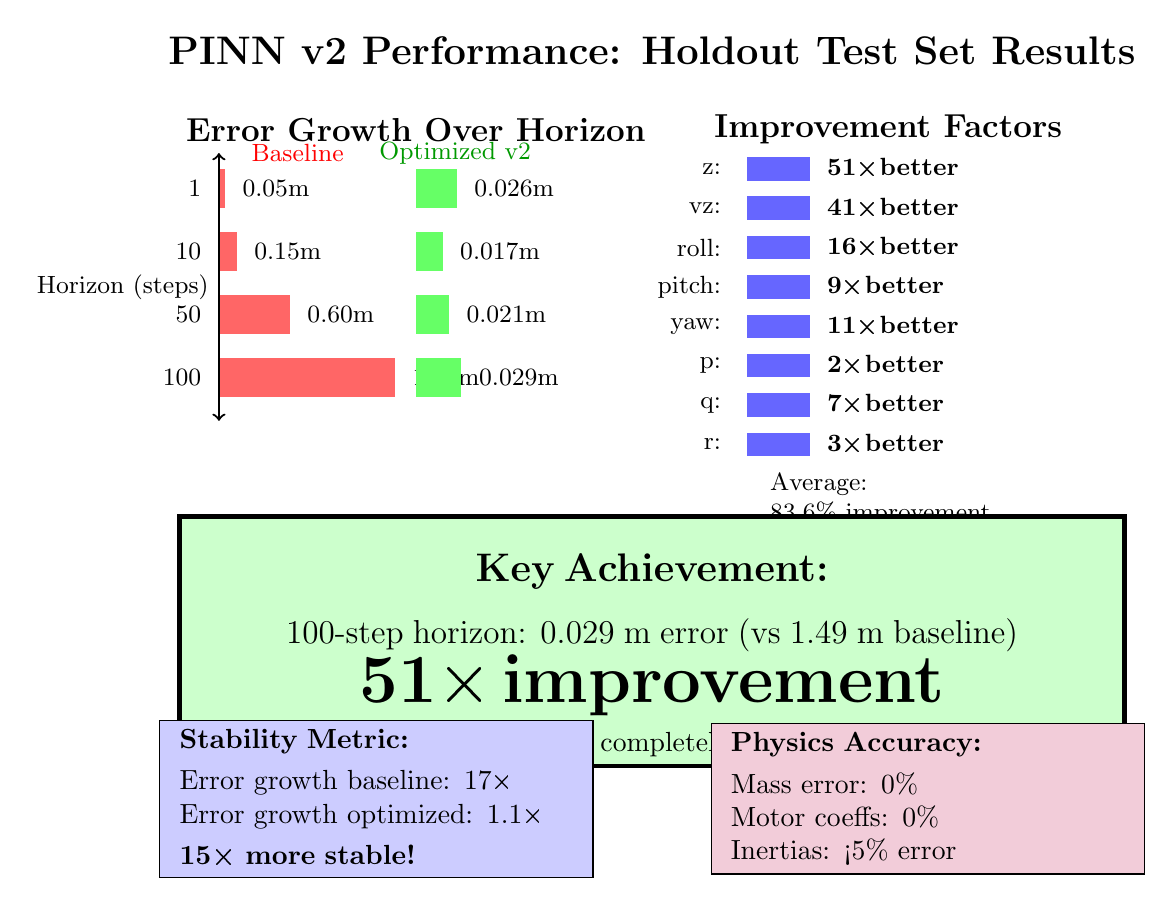
\begin{tikzpicture}

\node[font=\Large\bfseries] at (6,10) {PINN v2 Performance: Holdout Test Set Results};

% Error growth comparison
\node[font=\large\bfseries] at (3,9) {Error Growth Over Horizon};

% Baseline bars
\foreach \h/\err/\y in {1/0.05/8, 10/0.15/7.2, 50/0.60/6.4, 100/1.49/5.6} {
    \fill[red!60] (0.5,\y) rectangle (0.5+\err*1.5,\y+0.5);
    \node[right, font=\small] at (0.5+\err*1.5+0.1,\y+0.25) {\err m};
    \node[left, font=\small] at (0.4,\y+0.25) {\h};
}

% Optimized bars
\foreach \h/\err/\y in {1/0.026/8, 10/0.017/7.2, 50/0.021/6.4, 100/0.029/5.6} {
    \fill[green!60] (3,\y) rectangle (3+\err*20,\y+0.5);
    \node[right, font=\small] at (3+\err*20+0.1,\y+0.25) {\err m};
}

\node[font=\small] at (1.5,8.7) {\textcolor{red}{Baseline}};
\node[font=\small] at (3.5,8.7) {\textcolor{green!60!black}{Optimized v2}};

\draw[<->, thick] (0.5,5.3) -- (0.5,8.7) node[midway, left, font=\small] {Horizon (steps)};

% Improvement factors
\node[font=\large\bfseries] at (9,9) {Improvement Factors};

\foreach \state/\imp/\y in {z/51×/8.5, vz/41×/8, roll/16×/7.5, pitch/9×/7, yaw/11×/6.5, p/2×/6, q/7×/5.5, r/3×/5} {
    \node[left, font=\small] at (7,\y) {\state:};
    \fill[blue!60] (7.2,\y-0.15) rectangle (7.2+0.8,\y+0.15);
    \node[right, font=\small\bfseries] at (8.1,\y) {\imp better};
}

\node[font=\small, text width=3cm] at (9,4.3) {Average:\\83.6\% improvement};

% Key result box
\node[draw, ultra thick, fill=green!20, minimum width=12cm, minimum height=2cm, text width=11.5cm] at (6,2.5) {
    \begin{center}
    \textbf{\Large Key Achievement:}\\[0.3cm]
    \large 100-step horizon: 0.029 m error (vs 1.49 m baseline)\\
    \textbf{\Huge 51× improvement}\\[0.2cm]
    \normalsize Evaluated on 9,873 completely unseen timesteps
    \end{center}
};

% Stability metric
\node[draw, fill=blue!20, minimum width=5.5cm, minimum height=1.5cm, text width=5cm] at (2.5,0.5) {
    \textbf{Stability Metric:}\\[0.1cm]
    Error growth baseline: 17×\\
    Error growth optimized: 1.1×\\[0.1cm]
    \textbf{15× more stable!}
};

\node[draw, fill=purple!20, minimum width=5.5cm, minimum height=1.5cm, text width=5cm] at (9.5,0.5) {
    \textbf{Physics Accuracy:}\\[0.1cm]
    Mass error: 0\%\\
    Motor coeffs: 0\%\\
    Inertias: <5\% error
};

\end{tikzpicture}
\end{figure}

\end{document}
